\documentclass[12pt, a4paper]{article}
\usepackage{amsmath}
\usepackage{amssymb}
\usepackage{geometry}
\usepackage{graphicx}
\usepackage[american, siunitx]{circuitikz}
\usepackage{pgfplots}
\pgfplotsset{compat=1.18}
\usetikzlibrary{calc, fillbetween}
\usepackage[colorlinks=true, allcolors=black]{hyperref}

% Document Formatting
\geometry{a4paper, margin=1in}
\linespread{1.2}

\title{\textbf{Capacitor Crash Course \& Problem Solutions}}
\author{}
\date{\today}

\begin{document}
\maketitle
\tableofcontents
\newpage

\section{Capacitor Crash Course}

Welcome! This guide will quickly cover the essential concepts you need to solve problems involving capacitors.

\subsection{What is a Capacitor?}
A capacitor is a component that \textbf{stores electrical energy} in an electric field. Think of it like a small, rechargeable battery that can charge and discharge very quickly.

\begin{itemize}
    \item \textbf{How it works:} It consists of two conductive plates separated by an insulating material called a \textbf{dielectric}. When a voltage is applied, positive charge builds up on one plate and negative charge on the other.
    \item \textbf{Key Equation:} The relationship between charge ($Q$), voltage ($V$), and capacitance ($C$) is:
    $$ Q = CV $$
    Capacitance is measured in \textbf{Farads (F)}. A \SI{1}{\micro\farad} capacitor can store \SI{1}{\micro\coulomb} of charge for every 1 volt applied.
\end{itemize}

\subsection{The Parallel Plate Capacitor \& Dielectrics}
For a standard parallel plate capacitor, its capacitance depends on its geometry and the dielectric material between the plates.

\begin{itemize}
    \item \textbf{Capacitance Formula:}
    $$ C = \frac{\epsilon_0 A}{d} $$
    Where $A$ is the area of the plates, $d$ is the distance between them, and $\epsilon_0$ is the permittivity of free space (\SI{8.854e-12}{\farad\per\meter}).
    \item \textbf{Dielectrics:} Inserting an insulating material (a dielectric) between the plates \textbf{increases} the capacitance.
    \begin{itemize}
        \item The \textbf{dielectric constant ($\kappa$)} is a factor by which capacitance is multiplied.
        \item \textbf{New Capacitance:}
        $$ C' = \kappa C_{\text{original}} = \kappa \frac{\epsilon_0 A}{d} $$
    \end{itemize}
\end{itemize}
\begin{figure}[htbp]
\centering
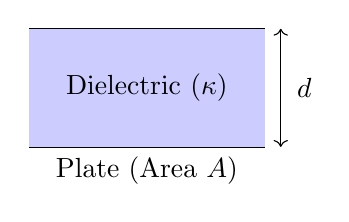
\begin{tikzpicture}
    % Plates
    \draw[thick] (0,0) -- (3,0);
    \draw[thick] (0,1.5) -- (3,1.5);
    \node at (1.5, -0.3) {Plate (Area $A$)};
    % Dielectric
    \fill[blue!20] (0,0) rectangle (3,1.5);
    \node at (1.5, 0.75) {Dielectric ($\kappa$)};
    % Annotation
    \draw[<->] (3.2,0) -- (3.2,1.5);
    \node at (3.5, 0.75) {$d$};
\end{tikzpicture}
\caption{A parallel plate capacitor with a dielectric.}
\end{figure}

\subsection{Combining Capacitors}
Just like resistors, capacitors can be combined in series and parallel.

\begin{itemize}
    \item \textbf{Capacitors in Parallel:}
    \begin{itemize}
        \item The voltage across each capacitor is the \textbf{same}.
        \item The total capacitance is the sum of individual capacitances.
        \item \textbf{Formula:} $C_{eq} = C_1 + C_2 + \dots$
        \item \textit{Think of it as increasing the total plate area.}
    \end{itemize}
    \begin{center}
    \begin{circuitikz}
        \draw (0,2) to[C=$C_1$] (2,2);
        \draw (0,0) to[C=$C_2$] (2,0);
        \draw (0,2) -- (0,0);
        \draw (2,2) -- (2,0);
    \end{circuitikz}
    \end{center}

    \item \textbf{Capacitors in Series:}
    \begin{itemize}
        \item The charge on each capacitor is the \textbf{same}.
        \item The reciprocals of the capacitances add up.
        \item \textbf{Formula:} $\frac{1}{C_{eq}} = \frac{1}{C_1} + \frac{1}{C_2} + \dots$
        \item \textit{Think of it as increasing the total plate separation distance.}
    \end{itemize}
    \begin{center}
    \begin{circuitikz}
        \draw (0,0) to[C=$C_1$] (2,0) to[C=$C_2$] (4,0);
    \end{circuitikz}
    \end{center}
\end{itemize}

\subsection{Capacitors in AC Circuits}
In an AC (alternating current) circuit, a capacitor continuously charges and discharges, effectively allowing current to flow. However, it offers opposition to this flow.

\begin{itemize}
    \item \textbf{Capacitive Reactance ($X_C$):} This is the "AC resistance" of a capacitor. It's measured in Ohms ($\Omega$).
    $$ X_C = \frac{1}{\omega C} = \frac{1}{2\pi f C} $$
    Where $f$ is the frequency of the AC supply in Hertz (Hz) and $\omega$ is the angular frequency.
    \item \textbf{Ohm's Law for AC:} The relationship between RMS voltage ($V_{rms}$), RMS current ($I_{rms}$), and reactance is just like Ohm's Law:
    $$ V_{rms} = I_{rms} X_C $$
\end{itemize}

\newpage

\section{Problem Walkthroughs \& Solutions}

\subsection{Problem 1: The Infinite Capacitor Network}
\noindent\textbf{Question:} An infinite capacitor network is connected to an AC voltage supply of \SI{220}{\volt}, \SI{50}{\hertz}. The capacitance of each capacitor is $C=\SI{1}{\micro\farad}$. Find the current through the ideal AC ammeter. Express your answer in terms of three significant figures.

\begin{figure}[htbp]
\centering
\begin{circuitikz}[scale=0.9]
    \draw (0,0) to[sV, l=\SI{220}{V} \SI{50}{Hz}] (0,3)
          to[ammeter] (1.5,3)
          to[C, l=$C$] (4,3)
          to[C, l=$C$] (6.5,3)
          to[C, l=$C$] (9,3);
    \draw (1.5,3) -- (1.5,1.5) to[C, l=$C$, mirror] (1.5,0);
    \draw (4,3) -- (4,1.5) to[C, l=$C$, mirror] (4,0);
    \draw (6.5,3) -- (6.5,1.5) to[C, l=$C$, mirror] (6.5,0);
    \draw (9,3) -- (9,1.5) to[C, l=$C$, mirror] (9,0);
    \draw (0,0) -- (1.5,0)
          to[C, l=$C$, mirror] (4,0)
          to[C, l=$C$, mirror] (6.5,0)
          to[C, l=$C$, mirror] (9,0);
    \draw[dashed, thick, ->] (9,3) -- (10.5,3);
    \draw[dashed, thick, ->] (9,0) -- (10.5,0);
    \node[align=center] at (10.5,1.5) {Repeat to \\ infinity...};
\end{circuitikz}
\caption{Infinite Capacitor Ladder Network.}
\end{figure}

\subsubsection*{Explanation \& Solution}
\begin{enumerate}
    \item \textbf{Set up the Self-Similarity Equation:}
    Let the equivalent capacitance of the entire network be $C_{eq}$. By its infinite nature, the network to the right of the first section is identical to the whole network, so its capacitance is also $C_{eq}$. The total capacitance is the first vertical capacitor ($C$) in parallel with the combination of the first top and bottom capacitors ($C$) and the rest of the network ($C_{eq}$), which are all in series. This gives the relation:
    $$ \frac{1}{C_{eq}} = \frac{2}{C} + \frac{1}{C+C_{eq}} $$
    Now, we solve for $C_{eq}$:
    $$ \frac{1}{C_{eq}} = \frac{2(C+C_{eq}) + C}{C(C+C_{eq})} $$
    $$ C(C+C_{eq}) = C_{eq}(3C + 2C_{eq}) $$
    $$ C^2 + C C_{eq} = 3C C_{eq} + 2C_{eq}^2 $$
    $$ 2C_{eq}^2 + 2C C_{eq} - C^2 = 0 $$

    \item \textbf{Solve for $C_{eq}$:}
    Using the quadratic formula $C_{eq} = \frac{-b \pm \sqrt{b^2 - 4ac}}{2a}$ with $a=2, b=2C, c=-C^2$:
    \begin{align*}
        C_{eq} &= \frac{-2C \pm \sqrt{(2C)^2 - 4(2)(-C^2)}}{4} \\
               &= \frac{-2C \pm \sqrt{4C^2 + 8C^2}}{4} \\
               &= \frac{-2C \pm 2\sqrt{3}C}{4}
    \end{align*}
    Since capacitance must be positive, we take the positive root:
    $$ C_{eq} = C \left( \frac{\sqrt{3}-1}{2} \right) $$
    Given $C = \SI{1}{\micro\farad} = \SI{1e-6}{\farad}$:
    $$ C_{eq} = (\SI{1e-6}{\farad}) \left( \frac{1.732 - 1}{2} \right) \approx \SI{0.366e-6}{\farad} $$

    \item \textbf{Calculate Total Capacitive Reactance ($X_{eq}$):}
    $$ X_{eq} = \frac{1}{2\pi f C_{eq}} = \frac{1}{2\pi (\SI{50}{\hertz})(\SI{0.366e-6}{\farad})} \approx \SI{8697}{\ohm} $$
    
    \item \textbf{Calculate the Current ($I$):}
    $$ I = \frac{V_{rms}}{X_{eq}} = \frac{\SI{220}{\volt}}{\SI{8697}{\ohm}} \approx \SI{0.0253}{\ampere} $$

\end{enumerate}
\textbf{Answer:} The current through the ammeter is \textbf{\SI{0.0253}{A}} (or \SI{25.3}{mA}).

\newpage

\subsection{Problem 2: Partially Inserted Dielectric}
\noindent\textbf{Question:} A parallel plate capacitor with the space between the plates filled with air has a capacitance of \SI{6}{\micro\farad}. It is charged by connecting to a \SI{24}{\volt} battery. With the capacitor still connected to the battery, an insulating material having dielectric constant of 2.5 is inserted into the space between the plates so that it fills exactly 50\% of the space. Calculate the amount of charge flowing through the battery during the process.

\subsubsection*{Explanation \& Solution}
\begin{enumerate}
    \item \textbf{Calculate the Initial Charge ($Q_i$):}
    $$ Q_i = C_i V = (\SI{6e-6}{\farad})(\SI{24}{\volt}) = \SI{144e-6}{\coulomb} = \SI{144}{\micro\coulomb} $$

    \item \textbf{Model the Final Capacitor:}
    When the dielectric is inserted, we can model this as two capacitors in \textbf{parallel}.
    \begin{itemize}
        \item \textbf{$C_{\text{air}}$:} Half the area, so $C_{\text{air}} = \frac{1}{2} C_i = \SI{3}{\micro\farad}$.
        \item \textbf{$C_{\text{dielectric}}$:} Half the area, times $\kappa$: $C_{\text{dielectric}} = \kappa \left(\frac{1}{2} C_i\right) = 2.5 \times \SI{3}{\micro\farad} = \SI{7.5}{\micro\farad}$.
    \end{itemize}

    \item \textbf{Calculate the Final Equivalent Capacitance ($C_f$):}
    $$ C_f = C_{\text{air}} + C_{\text{dielectric}} = \SI{3}{\micro\farad} + \SI{7.5}{\micro\farad} = \SI{10.5}{\micro\farad} $$
    
    \item \textbf{Calculate the Final Charge ($Q_f$):}
    $$ Q_f = C_f V = (\SI{10.5e-6}{\farad})(\SI{24}{\volt}) = \SI{252e-6}{\coulomb} = \SI{252}{\micro\coulomb} $$
    
    \item \textbf{Calculate the Charge Flow ($\Delta Q$):}
    $$ \Delta Q = Q_f - Q_i = \SI{252}{\micro\coulomb} - \SI{144}{\micro\coulomb} = \SI{108}{\micro\coulomb} $$
\end{enumerate}
\textbf{Answer:} The amount of charge flowing through the battery is \textbf{\SI{108}{\micro\coulomb}}.

\newpage

\subsection{Problem 3: Multiple Dielectrics}
\noindent\textbf{Question:} A parallel-plate capacitor is shown with plate area $A=\SI{10.5}{cm^2}$ and plate separation $2d=\SI{7.12}{mm}$. The gap is filled with three dielectrics: $\kappa_{1}=21.0$ (left half), $\kappa_{2}=42.0$ (top right), and $\kappa_{3}=58.0$ (bottom right). What is the capacitance?

\begin{figure}[htbp]
\centering
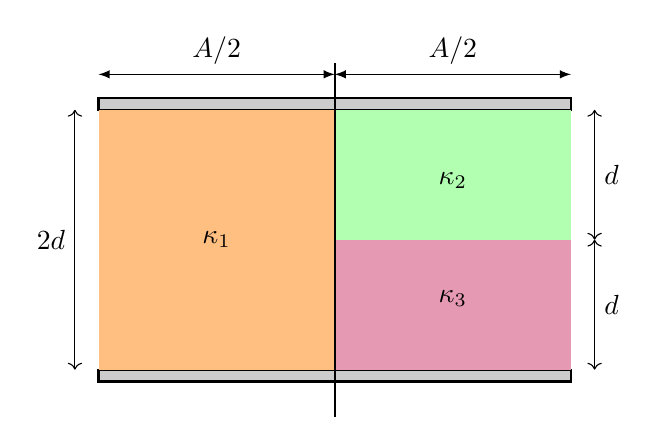
\begin{tikzpicture}[scale=1.5]
    % Plates
    \draw[fill=gray!40, thick] (-2,-1.1) rectangle (2,-1.2);
    \draw[fill=gray!40, thick] (-2,1.1) rectangle (2,1.2);
    % Dielectrics
    \fill[orange!50] (-2,-1.1) rectangle (0,1.1);
    \fill[green!30] (0,0) rectangle (2,1.1);
    \fill[purple!40] (0,0) rectangle (2,-1.1);
    % Labels
    \node at (-1,0) {$\kappa_1$};
    \node at (1,0.5) {$\kappa_2$};
    \node at (1,-0.5) {$\kappa_3$};
    % Dimensions
    \draw[<->] (-2.2, -1.1) -- (-2.2, 1.1) node[midway, left] {$2d$};
    \draw[<->] (2.2, 0) -- (2.2, 1.1) node[midway, right] {$d$};
    \draw[<->] (2.2, -1.1) -- (2.2, 0) node[midway, right] {$d$};
    \draw[<->, >=latex] (-2, 1.4) -- (0, 1.4) node[midway, above] {$A/2$};
    \draw[<->, >=latex] (0, 1.4) -- (2, 1.4) node[midway, above] {$A/2$};
    \draw[thick] (0,-1.5) -- (0,1.5);
\end{tikzpicture}
\caption{Capacitor with three different dielectric materials.}
\end{figure}

\subsubsection*{Explanation \& Solution}
\begin{enumerate}
    \item \textbf{Deconstruct the Capacitor:}
    Model this as three capacitors: $C_1$ (left half), $C_2$ (top-right), and $C_3$ (bottom-right). $C_2$ and $C_3$ are in series, and this combination ($C_{23}$) is in parallel with $C_1$.

    \item \textbf{Calculate Individual Capacitances:}
    \begin{align*}
        C_1 &= \kappa_1 \frac{\epsilon_0 (A/2)}{2d} = \frac{\kappa_1 \epsilon_0 A}{4d} \\
        C_2 &= \kappa_2 \frac{\epsilon_0 (A/2)}{d} = \frac{\kappa_2 \epsilon_0 A}{2d} \\
        C_3 &= \kappa_3 \frac{\epsilon_0 (A/2)}{d} = \frac{\kappa_3 \epsilon_0 A}{2d}
    \end{align*}

    \item \textbf{Combine the Series Part ($C_{23}$):}
    $$ \frac{1}{C_{23}} = \frac{1}{C_2} + \frac{1}{C_3} \implies C_{23} = \frac{\epsilon_0 A}{2d} \left( \frac{\kappa_2 \kappa_3}{\kappa_2 + \kappa_3} \right) $$

    \item \textbf{Combine for Total Capacitance ($C_{eq}$):}
    $$ C_{eq} = C_1 + C_{23} = \frac{\kappa_1 \epsilon_0 A}{4d} + \frac{\epsilon_0 A}{2d} \left( \frac{\kappa_2 \kappa_3}{\kappa_2 + \kappa_3} \right) $$
    Factoring out $\frac{\epsilon_0 A}{2d}$ gives the final expression:
    $$ C_{eq} = \frac{\epsilon_0 A}{2d} \left( \frac{\kappa_1}{2} + \frac{\kappa_2 \kappa_3}{\kappa_2 + \kappa_3} \right) $$
    
    \item \textbf{Substitute Values and Calculate:}
    Given: $A = \SI{10.5e-4}{m^2}$, $2d = \SI{7.12e-3}{m}$, $\kappa_1 = 21.0$, $\kappa_2 = 42.0$, $\kappa_3 = 58.0$.
    
    The pre-factor is:
    $$ \frac{\epsilon_0 A}{2d} = \frac{(\SI{8.854e-12}{F/m})(\SI{10.5e-4}{m^2})}{\SI{7.12e-3}{m}} \approx \SI{1.3057e-12}{F} $$
    The term in parentheses is:
    $$ \left( \frac{21.0}{2} + \frac{42.0 \times 58.0}{42.0 + 58.0} \right) = (10.5 + 24.36) = 34.86 $$
    The total capacitance is:
    $$ C_{eq} = (\SI{1.3057e-12}{F}) \times (34.86) \approx \SI{45.52e-12}{F} $$
\end{enumerate}
\textbf{Answer:} The capacitance is \textbf{\SI{45.5}{pF}} (picoFarads).

\end{document}